
% Default to the notebook output style

    


% Inherit from the specified cell style.




    
\documentclass{article}

    
    
    \usepackage{graphicx} % Used to insert images
    \usepackage{adjustbox} % Used to constrain images to a maximum size 
    \usepackage{color} % Allow colors to be defined
    \usepackage{enumerate} % Needed for markdown enumerations to work
    \usepackage{geometry} % Used to adjust the document margins
    \usepackage{amsmath} % Equations
    \usepackage{amssymb} % Equations
    \usepackage{eurosym} % defines \euro
    \usepackage[mathletters]{ucs} % Extended unicode (utf-8) support
    \usepackage[utf8x]{inputenc} % Allow utf-8 characters in the tex document
    \usepackage{fancyvrb} % verbatim replacement that allows latex
    \usepackage{grffile} % extends the file name processing of package graphics 
                         % to support a larger range 
    % The hyperref package gives us a pdf with properly built
    % internal navigation ('pdf bookmarks' for the table of contents,
    % internal cross-reference links, web links for URLs, etc.)
    \usepackage{hyperref}
    \usepackage{longtable} % longtable support required by pandoc >1.10
    \usepackage{booktabs}  % table support for pandoc > 1.12.2
    \usepackage{indentfirst}

    
    
    \definecolor{orange}{cmyk}{0,0.4,0.8,0.2}
    \definecolor{darkorange}{rgb}{.71,0.21,0.01}
    \definecolor{darkgreen}{rgb}{.12,.54,.11}
    \definecolor{myteal}{rgb}{.26, .44, .56}
    \definecolor{gray}{gray}{0.45}
    \definecolor{lightgray}{gray}{.95}
    \definecolor{mediumgray}{gray}{.8}
    \definecolor{inputbackground}{rgb}{.95, .95, .85}
    \definecolor{outputbackground}{rgb}{.95, .95, .95}
    \definecolor{traceback}{rgb}{1, .95, .95}
    % ansi colors
    \definecolor{red}{rgb}{.6,0,0}
    \definecolor{green}{rgb}{0,.65,0}
    \definecolor{brown}{rgb}{0.6,0.6,0}
    \definecolor{blue}{rgb}{0,.145,.698}
    \definecolor{purple}{rgb}{.698,.145,.698}
    \definecolor{cyan}{rgb}{0,.698,.698}
    \definecolor{lightgray}{gray}{0.5}
    
    % bright ansi colors
    \definecolor{darkgray}{gray}{0.25}
    \definecolor{lightred}{rgb}{1.0,0.39,0.28}
    \definecolor{lightgreen}{rgb}{0.48,0.99,0.0}
    \definecolor{lightblue}{rgb}{0.53,0.81,0.92}
    \definecolor{lightpurple}{rgb}{0.87,0.63,0.87}
    \definecolor{lightcyan}{rgb}{0.5,1.0,0.83}
    
    % commands and environments needed by pandoc snippets
    % extracted from the output of `pandoc -s`
    \providecommand{\tightlist}{%
      \setlength{\itemsep}{0pt}\setlength{\parskip}{0pt}}
    \DefineVerbatimEnvironment{Highlighting}{Verbatim}{commandchars=\\\{\}}
    % Add ',fontsize=\small' for more characters per line
    \newenvironment{Shaded}{}{}
    \newcommand{\KeywordTok}[1]{\textcolor[rgb]{0.00,0.44,0.13}{\textbf{{#1}}}}
    \newcommand{\DataTypeTok}[1]{\textcolor[rgb]{0.56,0.13,0.00}{{#1}}}
    \newcommand{\DecValTok}[1]{\textcolor[rgb]{0.25,0.63,0.44}{{#1}}}
    \newcommand{\BaseNTok}[1]{\textcolor[rgb]{0.25,0.63,0.44}{{#1}}}
    \newcommand{\FloatTok}[1]{\textcolor[rgb]{0.25,0.63,0.44}{{#1}}}
    \newcommand{\CharTok}[1]{\textcolor[rgb]{0.25,0.44,0.63}{{#1}}}
    \newcommand{\StringTok}[1]{\textcolor[rgb]{0.25,0.44,0.63}{{#1}}}
    \newcommand{\CommentTok}[1]{\textcolor[rgb]{0.38,0.63,0.69}{\textit{{#1}}}}
    \newcommand{\OtherTok}[1]{\textcolor[rgb]{0.00,0.44,0.13}{{#1}}}
    \newcommand{\AlertTok}[1]{\textcolor[rgb]{1.00,0.00,0.00}{\textbf{{#1}}}}
    \newcommand{\FunctionTok}[1]{\textcolor[rgb]{0.02,0.16,0.49}{{#1}}}
    \newcommand{\RegionMarkerTok}[1]{{#1}}
    \newcommand{\ErrorTok}[1]{\textcolor[rgb]{1.00,0.00,0.00}{\textbf{{#1}}}}
    \newcommand{\NormalTok}[1]{{#1}}
    
    % Define a nice break command that doesn't care if a line doesn't already
    % exist.
    \def\br{\hspace*{\fill} \\* }
    % Math Jax compatability definitions
    \def\gt{>}
    \def\lt{<}
    % Document parameters
    \title{Homework 4}
    \author{Roly Vicar\'ia \\ STAT501 Fall 2015}       
    
    

    % Pygments definitions
    
\makeatletter
\def\PY@reset{\let\PY@it=\relax \let\PY@bf=\relax%
    \let\PY@ul=\relax \let\PY@tc=\relax%
    \let\PY@bc=\relax \let\PY@ff=\relax}
\def\PY@tok#1{\csname PY@tok@#1\endcsname}
\def\PY@toks#1+{\ifx\relax#1\empty\else%
    \PY@tok{#1}\expandafter\PY@toks\fi}
\def\PY@do#1{\PY@bc{\PY@tc{\PY@ul{%
    \PY@it{\PY@bf{\PY@ff{#1}}}}}}}
\def\PY#1#2{\PY@reset\PY@toks#1+\relax+\PY@do{#2}}

\expandafter\def\csname PY@tok@gd\endcsname{\def\PY@tc##1{\textcolor[rgb]{0.63,0.00,0.00}{##1}}}
\expandafter\def\csname PY@tok@gu\endcsname{\let\PY@bf=\textbf\def\PY@tc##1{\textcolor[rgb]{0.50,0.00,0.50}{##1}}}
\expandafter\def\csname PY@tok@gt\endcsname{\def\PY@tc##1{\textcolor[rgb]{0.00,0.27,0.87}{##1}}}
\expandafter\def\csname PY@tok@gs\endcsname{\let\PY@bf=\textbf}
\expandafter\def\csname PY@tok@gr\endcsname{\def\PY@tc##1{\textcolor[rgb]{1.00,0.00,0.00}{##1}}}
\expandafter\def\csname PY@tok@cm\endcsname{\let\PY@it=\textit\def\PY@tc##1{\textcolor[rgb]{0.25,0.50,0.50}{##1}}}
\expandafter\def\csname PY@tok@vg\endcsname{\def\PY@tc##1{\textcolor[rgb]{0.10,0.09,0.49}{##1}}}
\expandafter\def\csname PY@tok@m\endcsname{\def\PY@tc##1{\textcolor[rgb]{0.40,0.40,0.40}{##1}}}
\expandafter\def\csname PY@tok@mh\endcsname{\def\PY@tc##1{\textcolor[rgb]{0.40,0.40,0.40}{##1}}}
\expandafter\def\csname PY@tok@go\endcsname{\def\PY@tc##1{\textcolor[rgb]{0.53,0.53,0.53}{##1}}}
\expandafter\def\csname PY@tok@ge\endcsname{\let\PY@it=\textit}
\expandafter\def\csname PY@tok@vc\endcsname{\def\PY@tc##1{\textcolor[rgb]{0.10,0.09,0.49}{##1}}}
\expandafter\def\csname PY@tok@il\endcsname{\def\PY@tc##1{\textcolor[rgb]{0.40,0.40,0.40}{##1}}}
\expandafter\def\csname PY@tok@cs\endcsname{\let\PY@it=\textit\def\PY@tc##1{\textcolor[rgb]{0.25,0.50,0.50}{##1}}}
\expandafter\def\csname PY@tok@cp\endcsname{\def\PY@tc##1{\textcolor[rgb]{0.74,0.48,0.00}{##1}}}
\expandafter\def\csname PY@tok@gi\endcsname{\def\PY@tc##1{\textcolor[rgb]{0.00,0.63,0.00}{##1}}}
\expandafter\def\csname PY@tok@gh\endcsname{\let\PY@bf=\textbf\def\PY@tc##1{\textcolor[rgb]{0.00,0.00,0.50}{##1}}}
\expandafter\def\csname PY@tok@ni\endcsname{\let\PY@bf=\textbf\def\PY@tc##1{\textcolor[rgb]{0.60,0.60,0.60}{##1}}}
\expandafter\def\csname PY@tok@nl\endcsname{\def\PY@tc##1{\textcolor[rgb]{0.63,0.63,0.00}{##1}}}
\expandafter\def\csname PY@tok@nn\endcsname{\let\PY@bf=\textbf\def\PY@tc##1{\textcolor[rgb]{0.00,0.00,1.00}{##1}}}
\expandafter\def\csname PY@tok@no\endcsname{\def\PY@tc##1{\textcolor[rgb]{0.53,0.00,0.00}{##1}}}
\expandafter\def\csname PY@tok@na\endcsname{\def\PY@tc##1{\textcolor[rgb]{0.49,0.56,0.16}{##1}}}
\expandafter\def\csname PY@tok@nb\endcsname{\def\PY@tc##1{\textcolor[rgb]{0.00,0.50,0.00}{##1}}}
\expandafter\def\csname PY@tok@nc\endcsname{\let\PY@bf=\textbf\def\PY@tc##1{\textcolor[rgb]{0.00,0.00,1.00}{##1}}}
\expandafter\def\csname PY@tok@nd\endcsname{\def\PY@tc##1{\textcolor[rgb]{0.67,0.13,1.00}{##1}}}
\expandafter\def\csname PY@tok@ne\endcsname{\let\PY@bf=\textbf\def\PY@tc##1{\textcolor[rgb]{0.82,0.25,0.23}{##1}}}
\expandafter\def\csname PY@tok@nf\endcsname{\def\PY@tc##1{\textcolor[rgb]{0.00,0.00,1.00}{##1}}}
\expandafter\def\csname PY@tok@si\endcsname{\let\PY@bf=\textbf\def\PY@tc##1{\textcolor[rgb]{0.73,0.40,0.53}{##1}}}
\expandafter\def\csname PY@tok@s2\endcsname{\def\PY@tc##1{\textcolor[rgb]{0.73,0.13,0.13}{##1}}}
\expandafter\def\csname PY@tok@vi\endcsname{\def\PY@tc##1{\textcolor[rgb]{0.10,0.09,0.49}{##1}}}
\expandafter\def\csname PY@tok@nt\endcsname{\let\PY@bf=\textbf\def\PY@tc##1{\textcolor[rgb]{0.00,0.50,0.00}{##1}}}
\expandafter\def\csname PY@tok@nv\endcsname{\def\PY@tc##1{\textcolor[rgb]{0.10,0.09,0.49}{##1}}}
\expandafter\def\csname PY@tok@s1\endcsname{\def\PY@tc##1{\textcolor[rgb]{0.73,0.13,0.13}{##1}}}
\expandafter\def\csname PY@tok@kd\endcsname{\let\PY@bf=\textbf\def\PY@tc##1{\textcolor[rgb]{0.00,0.50,0.00}{##1}}}
\expandafter\def\csname PY@tok@sh\endcsname{\def\PY@tc##1{\textcolor[rgb]{0.73,0.13,0.13}{##1}}}
\expandafter\def\csname PY@tok@sc\endcsname{\def\PY@tc##1{\textcolor[rgb]{0.73,0.13,0.13}{##1}}}
\expandafter\def\csname PY@tok@sx\endcsname{\def\PY@tc##1{\textcolor[rgb]{0.00,0.50,0.00}{##1}}}
\expandafter\def\csname PY@tok@bp\endcsname{\def\PY@tc##1{\textcolor[rgb]{0.00,0.50,0.00}{##1}}}
\expandafter\def\csname PY@tok@c1\endcsname{\let\PY@it=\textit\def\PY@tc##1{\textcolor[rgb]{0.25,0.50,0.50}{##1}}}
\expandafter\def\csname PY@tok@kc\endcsname{\let\PY@bf=\textbf\def\PY@tc##1{\textcolor[rgb]{0.00,0.50,0.00}{##1}}}
\expandafter\def\csname PY@tok@c\endcsname{\let\PY@it=\textit\def\PY@tc##1{\textcolor[rgb]{0.25,0.50,0.50}{##1}}}
\expandafter\def\csname PY@tok@mf\endcsname{\def\PY@tc##1{\textcolor[rgb]{0.40,0.40,0.40}{##1}}}
\expandafter\def\csname PY@tok@err\endcsname{\def\PY@bc##1{\setlength{\fboxsep}{0pt}\fcolorbox[rgb]{1.00,0.00,0.00}{1,1,1}{\strut ##1}}}
\expandafter\def\csname PY@tok@mb\endcsname{\def\PY@tc##1{\textcolor[rgb]{0.40,0.40,0.40}{##1}}}
\expandafter\def\csname PY@tok@ss\endcsname{\def\PY@tc##1{\textcolor[rgb]{0.10,0.09,0.49}{##1}}}
\expandafter\def\csname PY@tok@sr\endcsname{\def\PY@tc##1{\textcolor[rgb]{0.73,0.40,0.53}{##1}}}
\expandafter\def\csname PY@tok@mo\endcsname{\def\PY@tc##1{\textcolor[rgb]{0.40,0.40,0.40}{##1}}}
\expandafter\def\csname PY@tok@kn\endcsname{\let\PY@bf=\textbf\def\PY@tc##1{\textcolor[rgb]{0.00,0.50,0.00}{##1}}}
\expandafter\def\csname PY@tok@mi\endcsname{\def\PY@tc##1{\textcolor[rgb]{0.40,0.40,0.40}{##1}}}
\expandafter\def\csname PY@tok@gp\endcsname{\let\PY@bf=\textbf\def\PY@tc##1{\textcolor[rgb]{0.00,0.00,0.50}{##1}}}
\expandafter\def\csname PY@tok@o\endcsname{\def\PY@tc##1{\textcolor[rgb]{0.40,0.40,0.40}{##1}}}
\expandafter\def\csname PY@tok@kr\endcsname{\let\PY@bf=\textbf\def\PY@tc##1{\textcolor[rgb]{0.00,0.50,0.00}{##1}}}
\expandafter\def\csname PY@tok@s\endcsname{\def\PY@tc##1{\textcolor[rgb]{0.73,0.13,0.13}{##1}}}
\expandafter\def\csname PY@tok@kp\endcsname{\def\PY@tc##1{\textcolor[rgb]{0.00,0.50,0.00}{##1}}}
\expandafter\def\csname PY@tok@w\endcsname{\def\PY@tc##1{\textcolor[rgb]{0.73,0.73,0.73}{##1}}}
\expandafter\def\csname PY@tok@kt\endcsname{\def\PY@tc##1{\textcolor[rgb]{0.69,0.00,0.25}{##1}}}
\expandafter\def\csname PY@tok@ow\endcsname{\let\PY@bf=\textbf\def\PY@tc##1{\textcolor[rgb]{0.67,0.13,1.00}{##1}}}
\expandafter\def\csname PY@tok@sb\endcsname{\def\PY@tc##1{\textcolor[rgb]{0.73,0.13,0.13}{##1}}}
\expandafter\def\csname PY@tok@k\endcsname{\let\PY@bf=\textbf\def\PY@tc##1{\textcolor[rgb]{0.00,0.50,0.00}{##1}}}
\expandafter\def\csname PY@tok@se\endcsname{\let\PY@bf=\textbf\def\PY@tc##1{\textcolor[rgb]{0.73,0.40,0.13}{##1}}}
\expandafter\def\csname PY@tok@sd\endcsname{\let\PY@it=\textit\def\PY@tc##1{\textcolor[rgb]{0.73,0.13,0.13}{##1}}}

\def\PYZbs{\char`\\}
\def\PYZus{\char`\_}
\def\PYZob{\char`\{}
\def\PYZcb{\char`\}}
\def\PYZca{\char`\^}
\def\PYZam{\char`\&}
\def\PYZlt{\char`\<}
\def\PYZgt{\char`\>}
\def\PYZsh{\char`\#}
\def\PYZpc{\char`\%}
\def\PYZdl{\char`\$}
\def\PYZhy{\char`\-}
\def\PYZsq{\char`\'}
\def\PYZdq{\char`\"}
\def\PYZti{\char`\~}
% for compatibility with earlier versions
\def\PYZat{@}
\def\PYZlb{[}
\def\PYZrb{]}
\makeatother


    % Exact colors from NB
    \definecolor{incolor}{rgb}{0.0, 0.0, 0.5}
    \definecolor{outcolor}{rgb}{0.545, 0.0, 0.0}



    
    % Prevent overflowing lines due to hard-to-break entities
    \sloppy 
    % Setup hyperref package
    \hypersetup{
      breaklinks=true,  % so long urls are correctly broken across lines
      colorlinks=true,
      urlcolor=blue,
      linkcolor=darkorange,
      citecolor=darkgreen,
      }
    % Slightly bigger margins than the latex defaults
    
    \geometry{verbose,tmargin=1in,bmargin=1in,lmargin=1in,rmargin=1in}
    
    

    \begin{document}
    
    
    \maketitle
    
    

    
    \subsubsection{Question 1}\label{question-1}

\begin{enumerate}
\def\labelenumi{\alph{enumi})}
\item
  True. This means that the data points were evenly distributed above
  and below the line.
\item
  False. An ideal residual plot for a valid model should display
  residuals randomly scattered around the residual = 0 line.
\item
  True. We would want to see a horizontal ``band'' around the residual =
  0 line to show that error variances are equal.
\item
  False. We shold confirm the linearity and equal variance conditions
  first since those conditions can affect the normality.
\item
  False. It could be useful in determining whether or not to add another
  predictor to the model.
\item
  False. We may have independence and equal variance of error terms but
  still not fit the linear model.
\item
  False. We should question our model if any of the conditions seem in
  doubt. We may determine that the doubt is not significant in a given
  context, but that determination still needs to be made.
\item
  False. It is very subjective and needs to be considered in the context
  of the purpose for which the model was constructued.
\end{enumerate}

    \subsubsection{Question 2}\label{question-2}

\begin{enumerate}
\def\labelenumi{\alph{enumi})}
\item
  Based on the residuals plot, we can see that the residuals do not
  ``bounce randomly'' around the residual = 0 line. Instead it has
  positive values for smaller fitted values, close to 0. This calls into
  question the assumption that the relationship is linear. Also, the
  residuals don't form a ``horizontal band'' around the residual = 0
  line, which indicates that the variances of the error terms may not be
  equal.
\item
  Yes. Adding the new predictor has improved the residual plot. It shows
  more of ``random bounciness'' around the residual = 0 line. It's not
  ideal, but better than before.
\end{enumerate}

    \subsubsection{Question 3}\label{question-3}

In terms of linearity, it looks like the Japan data has the most
``random bouncing'' of points around the residual = 0 line. The USA data
seems to have negative residuals for lower fitted values, then goes
positive for middle fitted values, and then scatters for the higher
values. That indicates that the USA data may not be linear. The Europe
data seems moderately scattered around the residual = 0 line.

In terms of the response following normal distribution, the USA data has
the most normal histogram for the residuals. The Europe data looks
skewed right, and the Japan data looks slightly skewed left.

In terms of the errors having equal variances, I think the USA data
seems to be the most consistently distributed. The Japan data shows a
little bit of a ``megaphone'' shape which indicates that the variance
increases relative to the fitted value. The Europe data is not far off,
but has some areas of greater spread than others.

    \subsubsection{Question 4}\label{question-4}

\begin{enumerate}
\def\labelenumi{\alph{enumi})}
\item
  The data of height versus desired height appears to show a positive
  relationship between the two variables. As height increases, desired
  height appears to increase also. 
  
  \begin{figure}[h!]
 \centering
 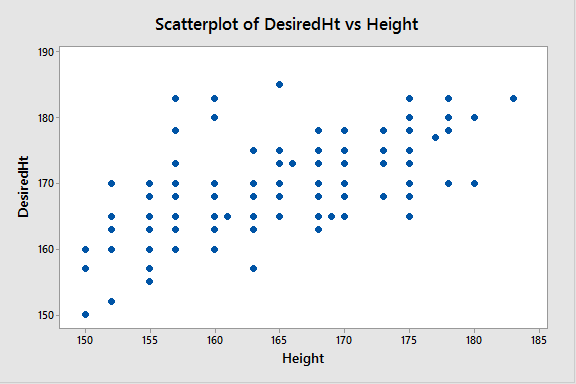
\includegraphics[scale=.5]{./images/scatterplot_height-vs-desiredHeight.png}
 % scatterplot_height-vs-desiredHeight.png: 576x384 pixel, 96dpi, 15.24x10.16 cm, bb=0 0 432 288
\end{figure}

\item
  \(DesiredHt = 77.84 + 0.5518 Height\)
\item
  The \(R^2\) value calculated by Minitab is 44.26\%. This value can be
  interpreted as saying that about 44\% of the variance in desired
  height is ``explained'' by the variation in actual height.
\item
  Some evidence supporting that the relationship is statistically
  significant is the \emph{t}-test for \(b_1\). The \emph{t}-value is
  14.06 which has a \emph{p}-value of 0.000. This is strong evidence
  that the desired height is positively correlated with actual height
  with slope \(b_1\).
  
\item
  The plot of residuals vs fitted values shows that the values appear to
  ``randomly bounce'' around the residual = 0 line. This supports the
  fit of the data to a linear model. The residuals also seem to
  distribute evenly around the residual = 0 line forming a ``horizontal
  band'' which indicates that the variance of the error terms is
  consistent. The only exception to the horizontal band are the
  appearance of a few potential outliers, 5 points with residual value
  greater than 10. 
  
  \begin{figure}[h!]
 \centering
 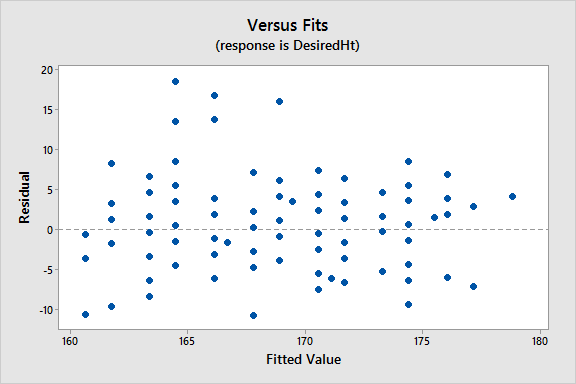
\includegraphics[scale=.5]{./images/plot-residuals-vs-fit_height-vs-desiredHeight.png}
 % plot-residuals-vs-fit_height-vs-desiredHeight.png: 576x384 pixel, 96dpi, 15.24x10.16 cm, bb=0 0 432 288
\end{figure}

  \newpage
\item
  The histogram confirms what we saw in the previous plot, namely that
  the residuals are fairly normal with only a few potential outliers
  with value greater than 12. The probability plot conveys this same
  observation. The probability plot shows the tail to the right. It's
  hard to say if this is a small departure from normality or a major
  departure. Aside from the 5 values on the right, it is a fairly
  straight line which indicates normality. It may not create significant
  problems.
  
  \begin{figure}[h!]
 \centering
 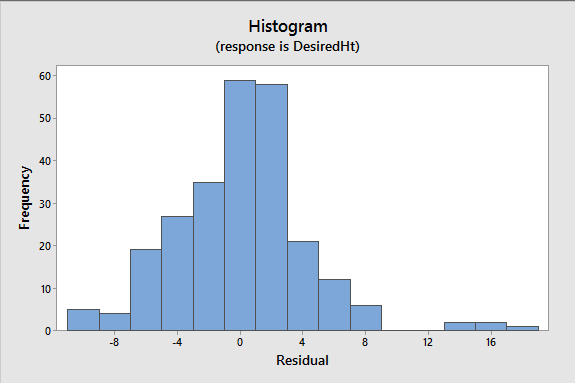
\includegraphics[scale=.5]{./images/histogram-residuals_height-vs-desiredHeight1.png}
 % histogram-residuals_height-vs-desiredHeight1.png: 575x383 pixel, 96dpi, 15.21x10.13 cm, bb=0 0 431 287
\end{figure}

\begin{figure}[h!]
 \centering
 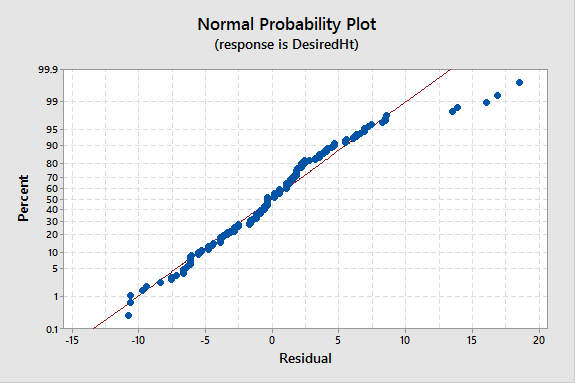
\includegraphics[scale=.5]{./images/probability-plot-residuals_height-vs-desiredHeight.png}
 % probability-plot-residuals_height-vs-desiredHeight.png: 575x383 pixel, 96dpi, 15.21x10.13 cm, bb=0 0 431 287
\end{figure}

\end{enumerate}

    \subsubsection{Question 5}\label{question-5}

\begin{enumerate}
\def\labelenumi{\alph{enumi})}
\item
\end{enumerate}

\begin{longtable}[c]{@{}llll@{}}
\toprule
Predictor variable & \emph{S}-value & \(R^2\) value & Slope
\emph{t}-statistic\tabularnewline
\midrule
\endhead
\(X_1\) & 1.06996 & 80.65\% & 14.14\tabularnewline
\(X_2\) & 1.01855 & 82.46\% & 15.02\tabularnewline
\(X_3\) & 1.01873 & 82.46\% & 15.02\tabularnewline
\(X_4\) & 1.01878 & 82.45\% & 15.02\tabularnewline
\bottomrule
\end{longtable}

Based solely on these values, I would say that the models for \(Y\) vs
\(X_2, X_3, X_4\) are essentially tied for ``best'', followed by \(X_1\)

\newpage
\begin{enumerate}
\def\labelenumi{\alph{enumi})}
\setcounter{enumi}{1}
\item
  The residual plot for model with \(X_1\) shows a strong ``horizontal
  band'' shape around the residual = 0 line, indicating good linearity
  fit. It shows a potential outlier with residual value around -3. The
  residuals seems to show a pretty constant variance around the residual
  = 0 line.
  
  \begin{figure}[h!]
 \centering
 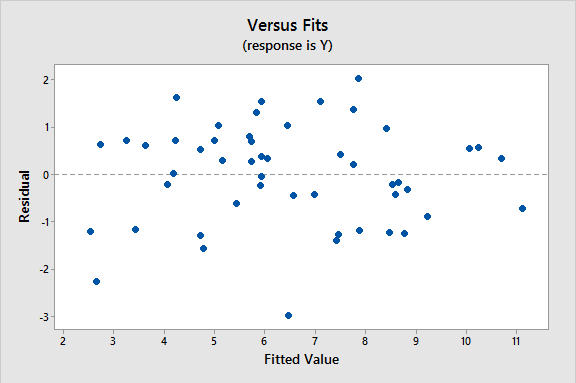
\includegraphics[scale=.3]{./images/plot-residuals-vs-fit_y-vs-x1.png}
 % plot-residuals-vs-fit_y-vs-x1.png: 576x383 pixel, 96dpi, 15.24x10.13 cm, bb=0 0 432 287
\end{figure}

\item
  The residual plot for model with \(X_2\) shows more of a ``megaphone''
  shape aronud the residual = 0 line. It also has some negative
  residuals for smaller fitted values. It calls into question the linear
  fit of the model. It also shows that the error variance grows for
  larger fitted values.
  
  \begin{figure}[h!]
 \centering
 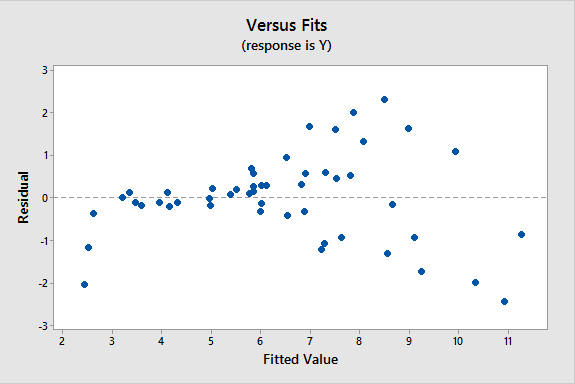
\includegraphics[scale=.3]{./images/plot-residuals-vs-fit_y-vs-x2.png}
 % plot-residuals-vs-fit_y-vs-x2.png: 575x384 pixel, 96dpi, 15.21x10.16 cm, bb=0 0 431 288
\end{figure}

\item
  The residual plot for the model with \(X_3\) also shows a possible
  lack of linear fit for the model. It shows some negative residuals for
  smaller fitted values, followed by a cluster of positive values,
  followed by a tail of more negative values. The variance of the error
  terms also does not look consistent.
  
  \begin{figure}[h!]
 \centering
 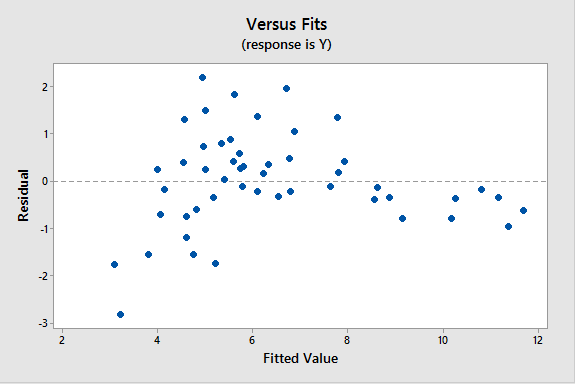
\includegraphics[scale=.3]{./images/plot-residuals-vs-fit_y-vs-x3.png}
 % plot-residuals-vs-fit_y-vs-x3.png: 575x384 pixel, 96dpi, 15.21x10.16 cm, bb=0 0 431 288
\end{figure}

\item
  The residual plot for model with \(X_4\) also shows lack of linear fit
  for the model. It shows two ``clusters'' of data points, the first
  with smaller fitted values, and another for larger fitted values. It
  appears that there may be another predictor value missing from the
  model to help explain \(Y\).
  
  \begin{figure}[h!]
 \centering
 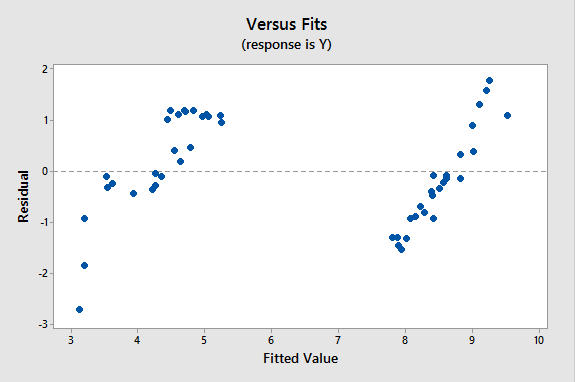
\includegraphics[scale=.3]{./images/plot-residuals-vs-fit_y-vs-x4.png}
 % plot-residuals-vs-fit_y-vs-x4.png: 575x382 pixel, 96dpi, 15.21x10.11 cm, bb=0 0 431 286
\end{figure}

\item
  Based on the residual vs fitted plots above, it would appear that the
  model with \(X_1\) would be the best one. It shows the best linear fit
  and most consistent variance for error terms with minimal number of
  outliers.
\end{enumerate}


    % Add a bibliography block to the postdoc
    
    
    
    \end{document}
